\section{TEST Data}




%------------------------------------------------
\begin{frame}[fragile]{Waveform: Unsynchronized}

Let:
\begin{itemize}
  \item The local clock inverts the GPIOA5 level state every 8ms. This test channel is marked CH\_LOCAL.

  \item The synchronous line generates a synchronous square wave with a half period of 8ms from the Master. This test channel is marked CH\_SYNC.

  \item In the interrupt processing function of the slave to capture the rising edge of the synchronization line, the clock is not synchronized, that is to say, the following code is commented out:

  \begin{lstlisting}
//dev.local_tm.jiffies = dev.local_tm.jiffies_pwm;		//synchronize code
  \end{lstlisting}

\end{itemize}

The following screenshots show the unsynchronized screenshots:


\end{frame}


%------------------------------------------------
\begin{frame}[fragile]{Waveform: Unsynchronized}

Unsynchronized waveform 1\label{nosyncwave1}:

  \begin{figure}[htbp]
  \begin{center}
  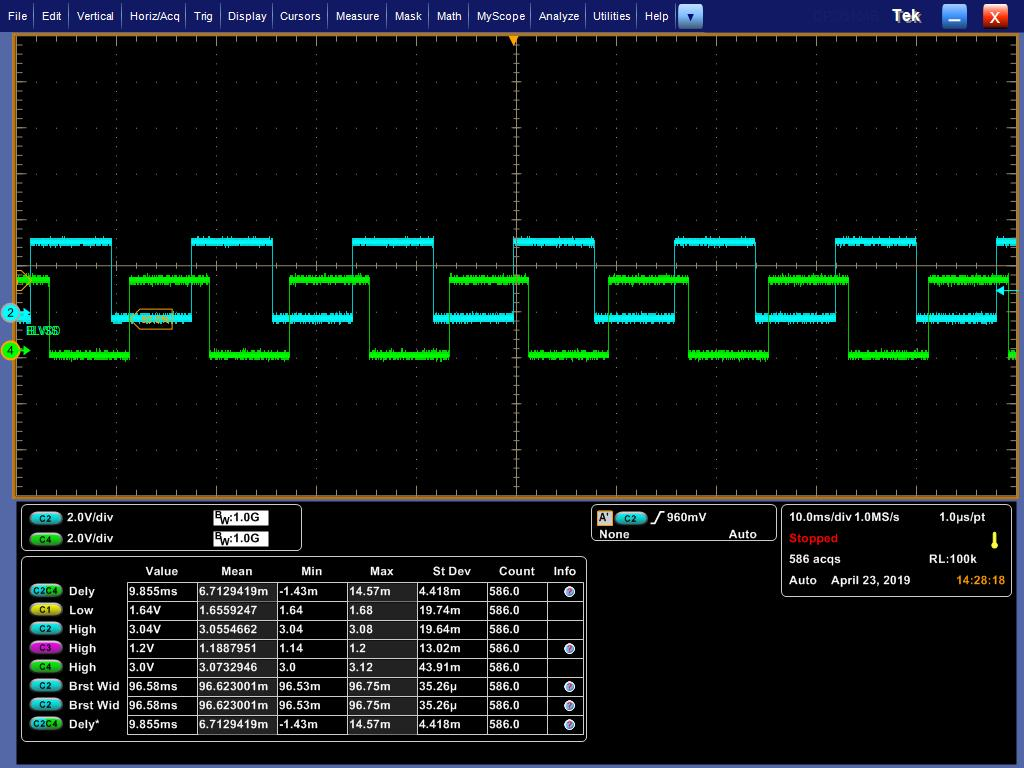
\includegraphics[width=10cm]{img/nosync1}
  \caption{nosync1}
  \label{report}
  \end{center}
  \vspace{-0.5em}
  \end{figure}


\end{frame}



%------------------------------------------------
\begin{frame}[fragile]{Waveform: Unsynchronized}

Unsynchronized waveform 2:

  \begin{figure}[htbp]
  \begin{center}
  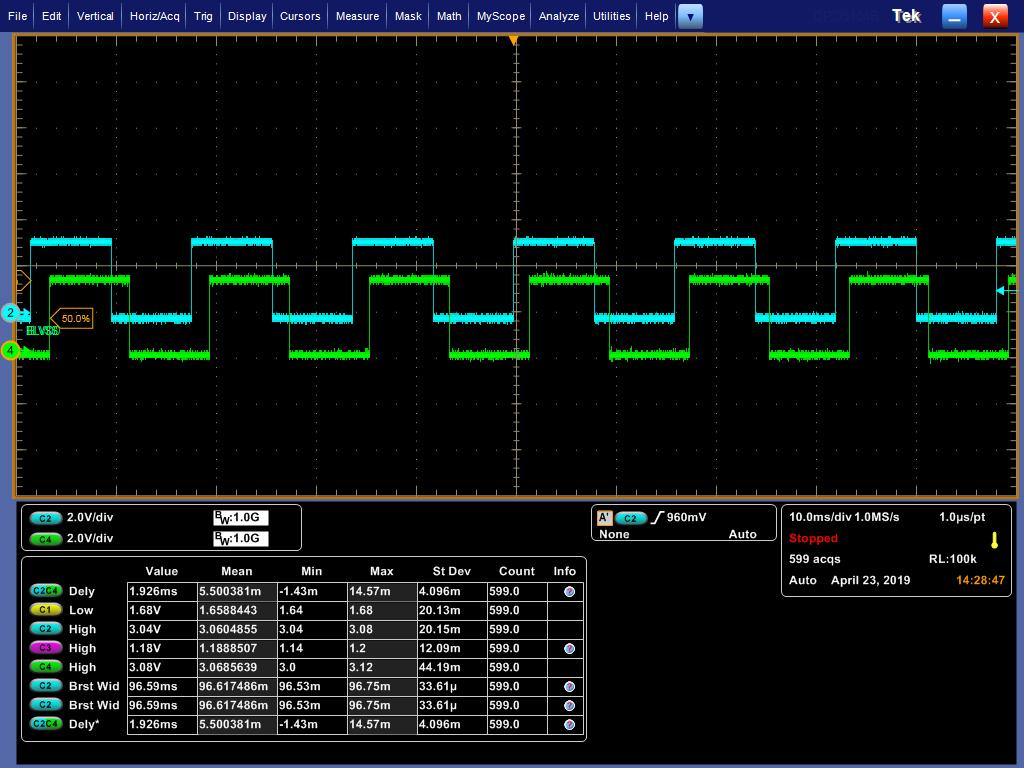
\includegraphics[width=10cm]{img/nosync2}
  \caption{nosync2}
  \label{report}
  \end{center}
  \vspace{-0.5em}
  \end{figure}


\end{frame}


%------------------------------------------------
\begin{frame}[fragile]{Waveform: Unsynchronized}

Unsynchronized waveform 3:

  \begin{figure}[htbp]
  \begin{center}
  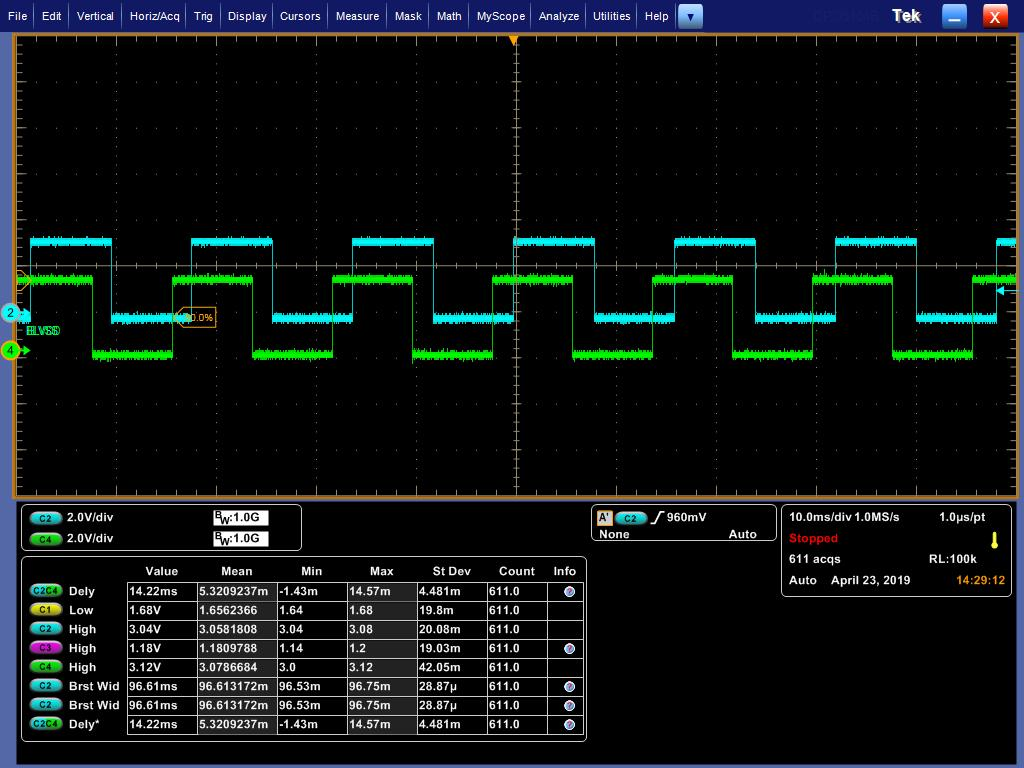
\includegraphics[width=10cm]{img/nosync3}
  \caption{nosync3}
  \label{report}
  \end{center}
  \vspace{-0.5em}
  \end{figure}


\end{frame}


%------------------------------------------------
\begin{frame}[fragile]{Waveform: Unsynchronized}

Unsynchronized waveform 4:

  \begin{figure}[htbp]
  \begin{center}
  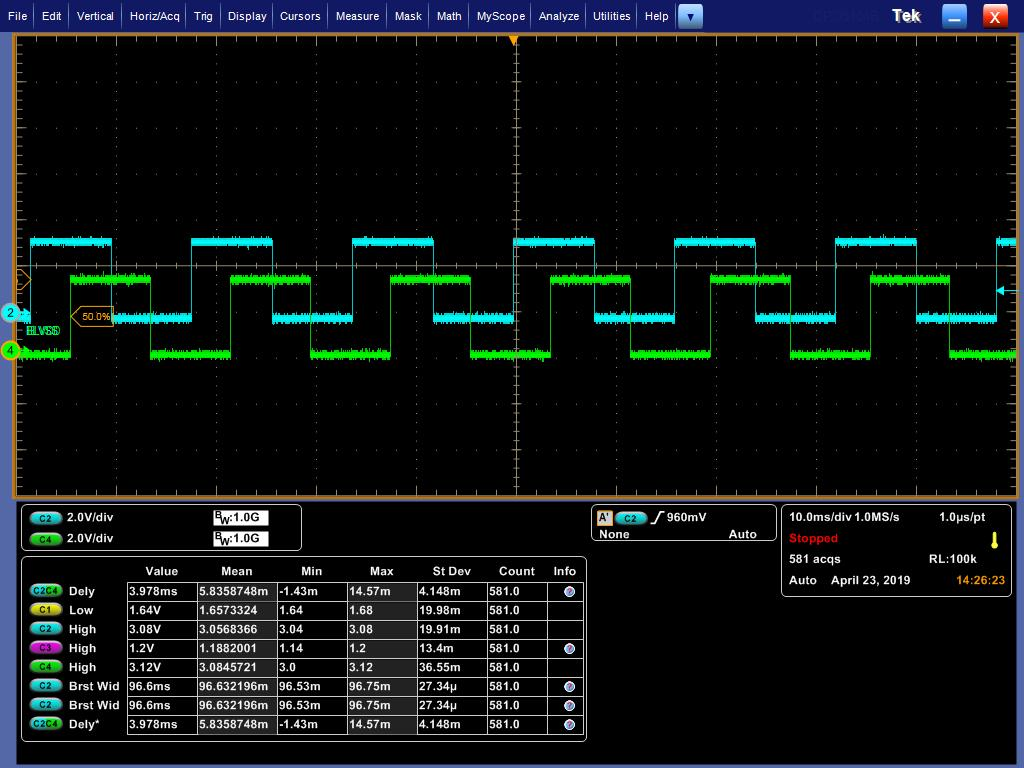
\includegraphics[width=10cm]{img/nosync4}
  \caption{nosync4}
  \label{report}
  \end{center}
  \vspace{-0.5em}
  \end{figure}


\end{frame}


%------------------------------------------------
\begin{frame}[fragile]{Some explanations of unsynchronized waveforms}


Return this document to unsynchronized waveform 1 ( \ref {nosyncwave1}) and turn the page with the right key of the keyboard direction key (from unsynchronized waveform 1 to unsynchronized waveform 4). At this time, the animation effect on the screen can restore the appearance of the oscilloscope at that time.

Because the local clock is not synchronized, each difference accumulates, resulting in such a dynamic effect.


\end{frame}



%------------------------------------------------
\begin{frame}[fragile]{Waveform: Synchronization }
Let:
\begin{itemize}
  \item The local clock inverts the GPIOA5 level state every 8ms. This test channel is marked CH\_LOCAL.

  \item The synchronous line generates a synchronous square wave with a half period of 8ms from the Master. This test channel is marked CH\_SYNC.
  \item In the interrupt processing function of the slave capturing the rising edge of the synchronization line, the clock is synchronized, that is to say, the following code is active:

  \begin{lstlisting}
dev.local_tm.jiffies = dev.local_tm.jiffies_pwm;		//synchronize code
  \end{lstlisting}

\end{itemize}

The following screenshots show the screenshots in the case of synchronization.

\end{frame}


%------------------------------------------------
\begin{frame}[fragile]{Waveform: Synchronization}

synchronized waveform :

  \begin{figure}[htbp]
  \begin{center}
  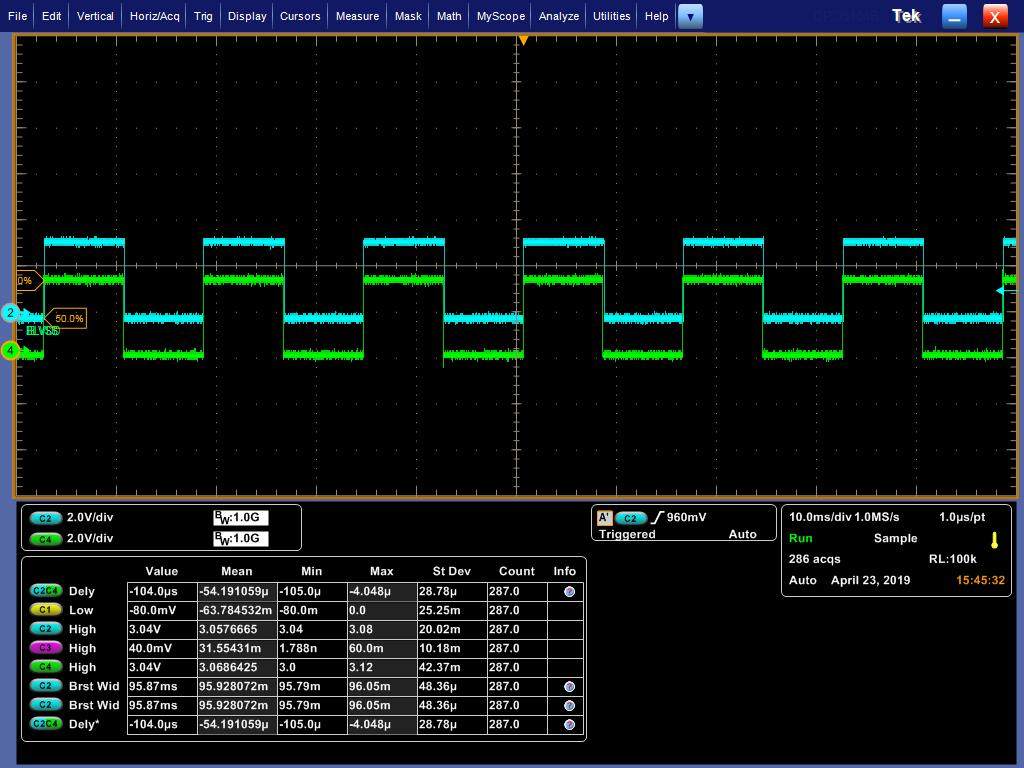
\includegraphics[width=10cm]{img/sync}
  \caption{report jiffies}
  \label{report}
  \end{center}
  \vspace{-0.5em}
  \end{figure}


\end{frame}

%------------------------------------------------
\begin{frame}[fragile]{Waveform: Synchronization}

Since the rising edge of each synchronization line is captured by slave computer, synchronization interrupt will be triggered. In interrupt processing, the local clock error of each cycle will be eliminated.


So the synchronized waveform looks fixed  and the phase is relatively consistent. But:

If we amplify the size of the oscilloscope, we will find that there are difference. The following are some synchronization delay. The size of the oscilloscope is already 50us. We are concerned about the synchronization time.


\end{frame}



%------------------------------------------------
\begin{frame}[fragile]{Waveform: Synchronization}

Synchronization delay:

  \begin{figure}[htbp]
  \begin{center}
  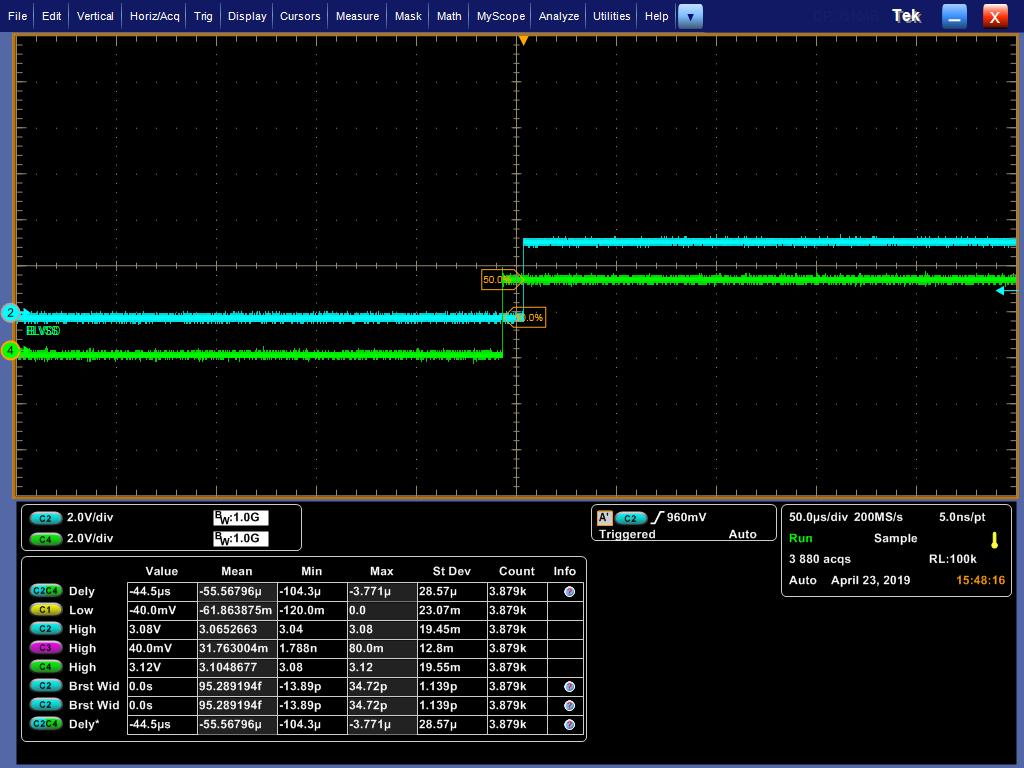
\includegraphics[width=10cm]{img/mis1}
  \caption{Synchronization delay1}
  \label{report}
  \end{center}
  \vspace{-0.5em}
  \end{figure}


\end{frame}


%------------------------------------------------
\begin{frame}[fragile]{Synchronization delay}

Synchronization delay:

  \begin{figure}[htbp]
  \begin{center}
  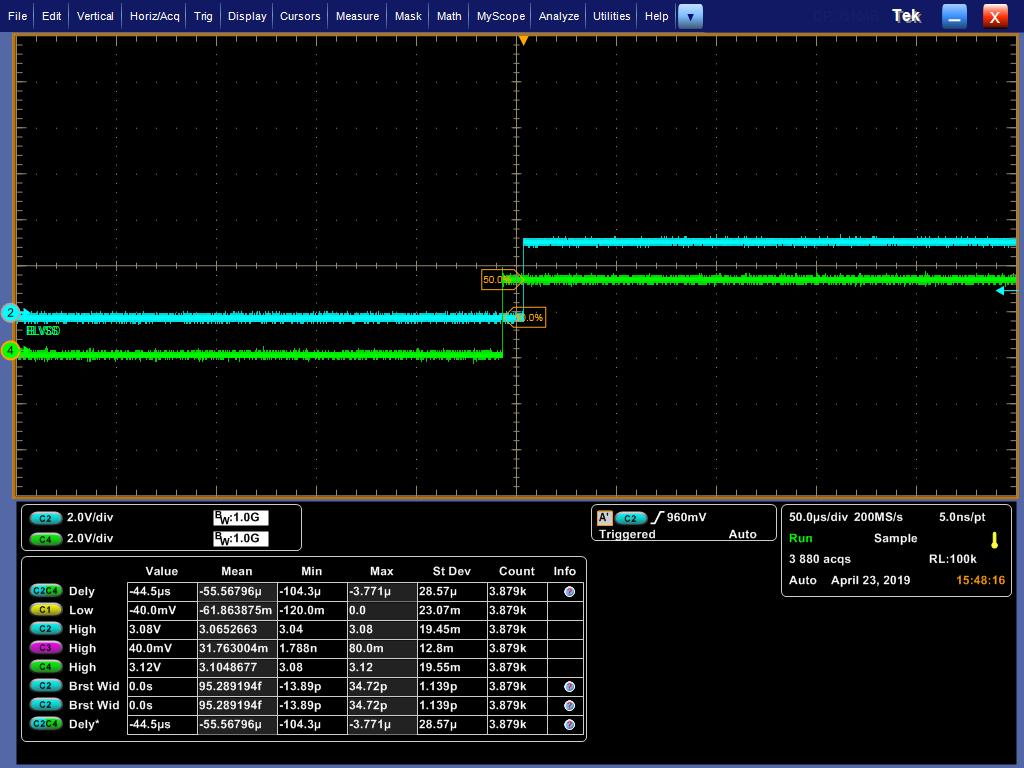
\includegraphics[width=10cm]{img/mis1}
  \caption{Synchronization delay1}
  \label{report}
  \end{center}
  \vspace{-0.5em}
  \end{figure}


\end{frame}
%------------------------------------------------
\begin{frame}[fragile]{Synchronization delay}

Synchronization delay:

  \begin{figure}[htbp]
  \begin{center}
  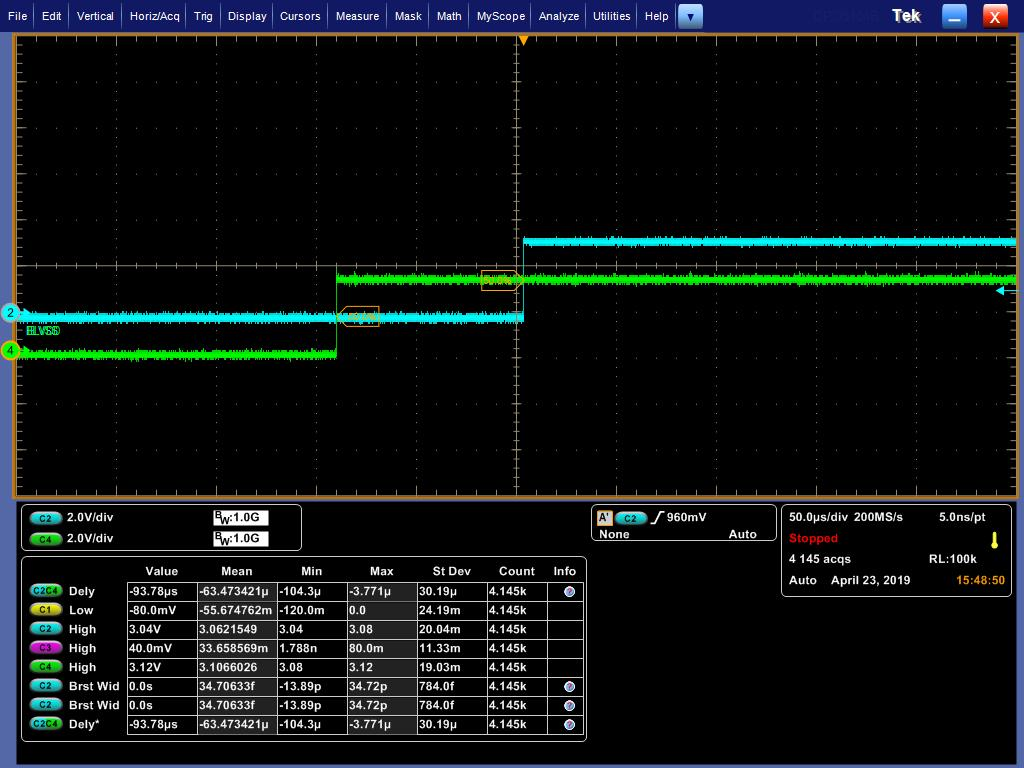
\includegraphics[width=10cm]{img/mis2}
  \caption{Synchronization delay2}
  \label{report}
  \end{center}
  \vspace{-0.5em}
  \end{figure}


\end{frame}

%------------------------------------------------
\begin{frame}[fragile]{Synchronization delay}

Synchronization delay:

  \begin{figure}[htbp]
  \begin{center}
  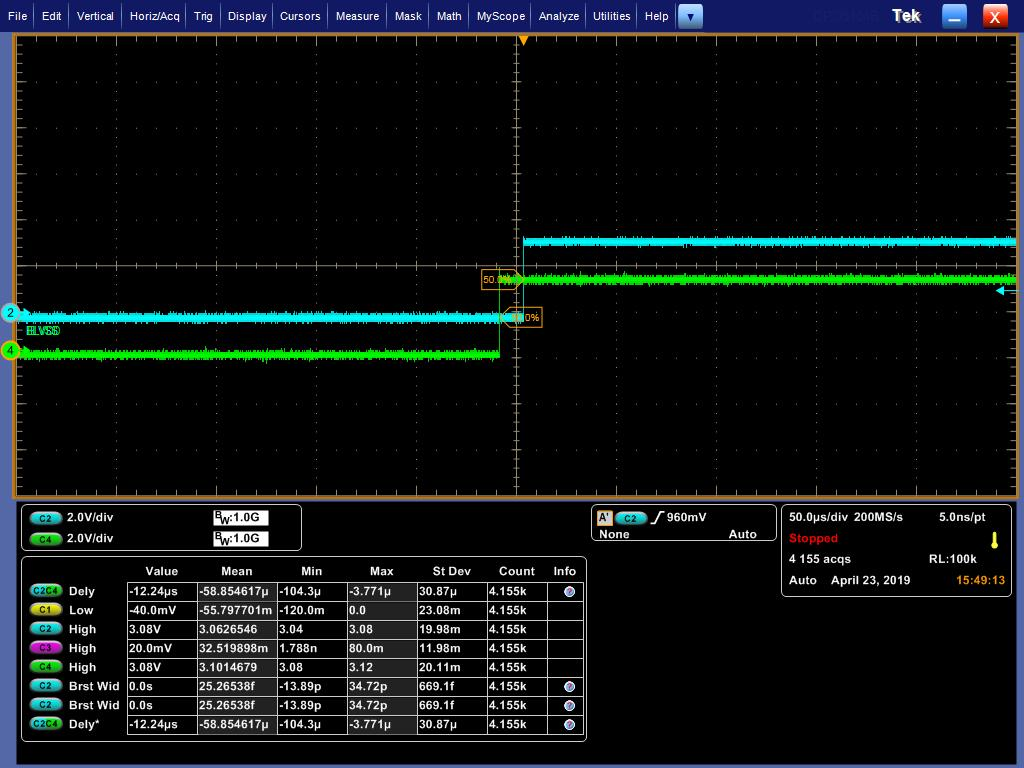
\includegraphics[width=10cm]{img/mis3}
  \caption{Synchronization delay3}
  \label{report}
  \end{center}
  \vspace{-0.5em}
  \end{figure}

\end{frame}


%------------------------------------------------
\begin{frame}[fragile]{Synchronization delay}

  \begin{figure}[htbp]
  \begin{center}
  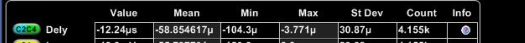
\includegraphics[width=7cm]{img/delay}
  \caption{delay}
  \label{report}
  \end{center}
  \vspace{-0.5em}
  \end{figure}


As can be seen from the figure above, the maximum phase difference between CH\_LOCAL and CH\_SYNC is -3.771 -(-104.3) = 100.529us  when sampling 4.155k times.

\end{frame}


%------------------------------------------------
\begin{frame}[fragile]{summary}

Data transmission through serial ports can cause some delays (although there is no blocking at the time of sending, receiving in the interrupt, reading registers directly). The baudrate we used in this example is 115200*2 bps.



Software-only CRC verification will inevitably lead to a certain delay. If it is necessary to verify, the driver of CRC hardware peripherals should be realized in this project.

The error of demo synchronization has been tested many times, among which there are transformed master-slave roles, and the maximum error is less than 500 us. The most common is within 300us.

The test code logic is not complex, real-time processing is in the interrupt context, and STM32F4 uses Cortex M4's Nested Vectored Interrupt Controller (NVIC) real-time is very high, there should be little optimization space.

\end{frame}
